    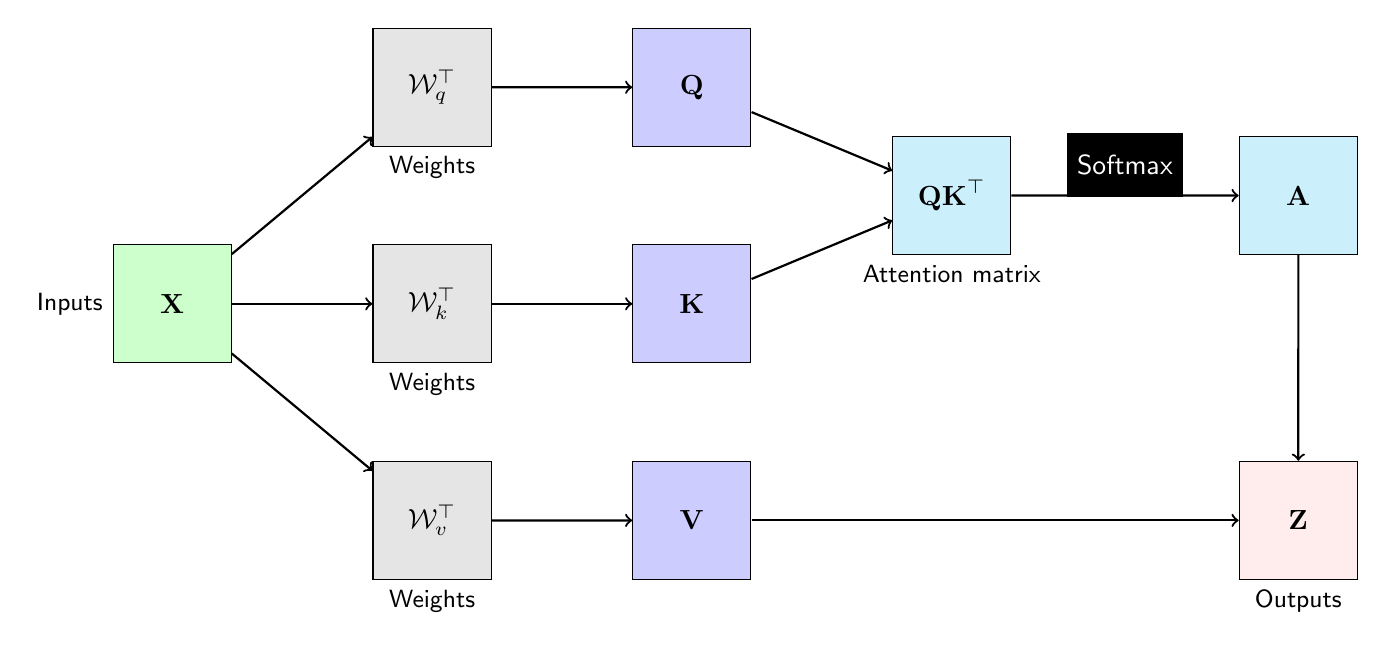
\begin{tikzpicture}[every node/.style={font=\sffamily, align=center}, box/.style={draw, minimum height=1.5cm, minimum width=1.5cm}, scale=1.1]
        % Input X
        \node[box, fill=green!20, label=left:{\small Inputs}] (x) at (0,0) {$\mathbf{X}$};

        % Weights
        \node[box, fill=gray!20, label=below:{\small Weights}] (wq) at (3,2.5) {$\mathcal{W}_q^\top$};
        \node[box, fill=gray!20, label=below:{\small Weights}] (wk) at (3,0) {$\mathcal{W}_k^\top$};
        \node[box, fill=gray!20, label=below:{\small Weights}] (wv) at (3,-2.5) {$\mathcal{W}_v^\top$};

        % Q, K, V
        \node[box, fill=blue!20] (q) at (6,2.5) {$\mathbf{Q}$};
        \node[box, fill=blue!20] (k) at (6,0) {$\mathbf{K}$};
        \node[box, fill=blue!20] (v) at (6,-2.5) {$\mathbf{V}$};

        % Attention matrix
        \node[box, fill=cyan!20, label=below:{\small Attention matrix}] (qk) at (9,1.25) {$\mathbf{QK}^\top$};
        \node[box, fill=cyan!20] (a) at (13,1.25) {$\mathbf{A}$};
        \node[draw, fill=black, text=white, minimum width=1.2cm, minimum height=0.8cm] at (11, 1.6) {Softmax};

        % Output Z
        \node[box, fill=pink!30, label=below:{\small Outputs}] (z) at (13, -2.5) {$\mathbf{Z}$};

        % Connections
        \draw[->, thick] (x) -- (wq);
        \draw[->, thick] (x) -- (wk);
        \draw[->, thick] (x) -- (wv);

        \draw[->, thick] (wq) -- (q);
        \draw[->, thick] (wk) -- (k);
        \draw[->, thick] (wv) -- (v);

        \draw[->, thick] (q) -- (qk);
        \draw[->, thick] (k) -- (qk);
        \draw[->, thick] (qk) -- (a);
        \draw[->, thick] (a) -- (z);
        \draw[->, thick] (v) -- (z);
    \end{tikzpicture}